%
%
%
\labelchapter{refcells}{Reference cells and side-effects}

Most of the values we have seen so far, like tuples and lists, are \emph{immutable}.  That is, once
a value is created, it never changes.  In this chapter we introduce operations and values for
imperative programming---programming with assignment, side-effects, and mutable state.

\label{keyword::=}
\index{reference cells}
\index{ref@\lstinline/ref/}
\index{!@\lstinline/!/ deference}
\index{:=@\lstinline/:=/ assignment}
The principal tool for imperative programming in OCaml is the \emph{reference cell}, which can be
viewed as a kind of ``box.''  The box always holds a value, but the contents of the box can be
replaced by assignment.  The operations on reference cells are as follows.

\begin{ocaml}
val ref  : 'a -> 'a ref
val (:=) : 'a ref -> 'a -> unit
val (!)  : 'a ref -> 'a
\end{ocaml}
%
Reference cells are created with the expression \hbox{\lstinline/ref e/}, which takes the initial
value \hbox{\lstinline/e/} for the reference cell.  The expression \hbox{\lstinline/!r/} returns the value in the
reference cell \hbox{\lstinline/r/}, and the expression \hbox{\lstinline/r := e/} replaces the contents of the
reference cell with the value \hbox{\lstinline/e/}.

\begin{figure}[t]
\begin{center}
\begin{tabular}{c|c}
Imperative factorial in C++ & Imperative factorial in OCaml\\
\hline\hline
\begin{clisting}
int factorial(int i) {
    int j = 1;
    for(int k = 2; k <= i; k++)
        j *= k;
    return j;
}
\end{clisting}
&
{\lstset{numbers=left,numberstyle=\tiny,firstnumber=1,stepnumber=1}
\begin{ocamllisting}
let factorial i =
    let j = ref 1 in
    for k := 2 to i do
       j := !j * k
    done;
    !j
\end{ocamllisting}}
\end{tabular}
\end{center}
\caption{Imperative implementations of a factorial function.}
\label{figure:imp-fact}
\end{figure}

For illustration, two imperative implementations of a factorial function are shown in
Figure~\ref{figure:imp-fact}, one written in C++, and the other in OCaml.  The structure of the code
is similar: the variable \hbox{\lstinline/j/} is initially defined to be \hbox{\lstinline/1/} on line 2;
then \hbox{\lstinline/j/} is multiplied by each value $2, \ldots, i$ on the for-loop in lines 3 and
4 to produce the final value $j = 1 * 2 * \cdots * i = i!$.

Structurally, the programs look quite similar, but there is a key difference in regard to the
variables.  In C, the variable \hbox{\lstinline/j/} is assigned to directly.  In OCaml, variables are
always immutable.  Instead, the variable \hbox{\lstinline/j/} refers to a reference cell and it is the
contents of the reference cell that is modified.  This also means that every time the value of the
cell is needed, the expression \hbox{\lstinline/!j/} is used.

\index{;!sequencing}
\label{keyword:;(sequencing)}
The figure also shows examples of sequencing and looping.  In OCaml, semicolons are used as
separators to specify sequencing of evaluation \hbox{\lstinline/$\nt{expression}_1$; $\nt{expression}_2$/}.
To evaluate the sequence, expression $\nt{expression}_1$ is first evaluated, the value discarded,
then the expression $\nt{expression}_2$ is evaluated and the value returned as the result of the
sequence.  It should be emphasized that the semicolon \hbox{\lstinline/;/} is not a terminator, like
it is in C.  For example, if line 6 of the OCaml factorial were followed by a semicolon, it would
mean that the value of the expression \hbox{\lstinline/!j/} should be discarded---and the value of the
function is defined by whatever follows the semicolon.

\index{loops}
\index{for-loop}
\index{while-loop}
\label{keyword:while}
\label{keyword:for}
\label{keyword:do}
\label{keyword:done}
\label{keyword:to}
\label{keyword:downto}
For-loops and while-loops are specified in one of the following forms.

\begin{ocaml}
for $\nt{identifier} := \nt{expression}_1$ to $\nt{expression}_2$ do $\nt{expression}_3$ done
for $\nt{identifier} := \nt{expression}_1$ downto $\nt{expression}_2$ do $\nt{expression}_3$ done
while $\nt{expression}_1$ do $\nt{expression}_2$ done
\end{ocaml}
%
In a for-loop, the body $\nt{expression}_3$ of the loop is evaluated for each value of the identifier
$\nt{identifier}$ between $\nt{expression}_1$ and $\nt{expression}_2$ inclusive; the \hbox{\lstinline/to/}
form counts upward by 1, and \hbox{\lstinline/downto/} counts down.  The expressions $\nt{expression}_1$
and $\nt{expression}_2$ are evaluated once, before the loop is entered.

A while-loop is evaluated by first evaluating the Boolean
expression $\nt{expression}_1$; if true, then the expression $\nt{expression}_2$ is evaluated for
its side-effect.  The evaluation is repeated until $\nt{expression}_1$ is false.  For comparison,
the factorial is implemented with a while-loop in Figure~\ref{figure:imp-fact2}.

\labelsection{pure-functional-programming}{Pure functional programming}

The one feature that is central to all functional programming languages is that functions are first
class values.  Functions can be passed as arguments and stored in data structures, just
like any other kind of value.  In fact, this is the only strict requirement for a language to be
functional, and by this definition it can be argued that many languages are functional, including C,
Javascript, OCaml, and others.

\index{pure functional programming}
A related property is \emph{purity}; a pure functional language does not include assignment or other
side-effects.  Haskell is an example of a pure functional language; OCaml and most Lisp dialects are
impure, meaning that they allow side-effects of some form.  One reason to prefer purity is that it
simplifies reasoning about programs.  In mathematics, a \emph{function} is defined as a
single-valued map, meaning that if $f$ is a function and $f(x)$ is defined for some $x$, then there
is only one value of $f(x)$.  Now, consider the following ``function'' written in C.

\begin{ccode}
int index = 1;
int g(int i) {
   index = index + 1;
   return i + index;
}
\end{ccode}
%
When called, the function modifies the variable \hbox{\lstinline/index/} by side-effect.  Mathematically
speaking, it is not a function because an expression like \hbox{\lstinline/g(0)/} can have many
possible values---in fact, the expression \hbox{\lstinline/g(0) == g(0)/} is always false!

\begin{figure}[t]
\begin{center}
\begin{tabular}{c|c}
Imperative factorial in C++ & Imperative factorial in OCaml\\
\hline\hline
\begin{clisting}
int factorial(int i) {
    int j = 1;
    while(i > 0) {
        j *= i;
        i--;
    }
    return j;
}
\end{clisting}
&
\begin{ocamllisting}
let factorial i =
    let j = ref 1 in
    let i = ref i in
    while !i > 0 do
       j := !j * !i;
       i := !i - 1
    done;
    !j
\end{ocamllisting}
\end{tabular}
\end{center}
\caption{Imperative implementations of a factorial function using while-loops.}
\label{figure:imp-fact2}
\end{figure}

\index{referential transparency}
Reasoning about imperative programs can be more difficult than it is for pure functional programs
because of the need to analyze the program state.  Pure functional programs don't have a global
mutable state, which simplifies their analysis.  More precisely, pure functional programs
provide \emph{referential transparency}, meaning that if two expressions evaluate to the same value,
then one can be substituted for the other without affecting the result of the computation.  For
example, consider an expression \hbox{\lstinline/f(0) + f(0)/}.  If the expression \hbox{\lstinline/f(0)/} is
referentially transparent, then the two occurrences can be replaced with the same value, and the
expression \hbox{\lstinline/let x = f(0) in x + x/} is equivalent (and probably more efficient).

Pure functional programming and referential transparency have many benefits.  Data structures are
persistent, meaning that once a data value is created, it cannot be changed or destroyed.  Programs
can be easier to reason about than equivalent imperative programs, and the compiler is given a great
deal of latitude in optimizations.

However, purity does have its drawbacks.  Side-effects can be useful in reducing code size.  For
example, suppose we have written a program containing a function \hbox{\lstinline/f(x)/}.  During testing,
we might want to know whether \hbox{\lstinline/f/} is ever called.  With side-effects, this is easy---we
add a flag that gets set whenever the function is called.  No other part of the program need be
changed.

\begin{ocaml}
let f_was_called = ref false

let f x =
   f_was_called := true;
   ...
\end{ocaml}
%
Without side-effects, this would be difficult to do without changing other parts of the program as
well.

Another, deeper, issue with purity is that it becomes impossible to construct some cyclic data
structures, ruling out some commonly-used data representations for graphs, circular
lists, \emph{etc}.  The problem is that, when a data value like a tuple or list is constructed, the
values it refers to must already exist.  In particular, a value being constructed may not, in
general, refer to itself.  In imperative programming, this is not an issue, because data values can be
constructed, then later mutated if a cyclic structure is desired.

A related issue is that, for some algorithms, the best known implementations are imperative.  For
these reasons, and perhaps others, OCaml supports side-effects, including operations on mutable data
and imperative input/output operations.  In the next few sections, we'll look at some common
imperative data representations using reference cells.

\labelsubsection{ref-value-restriction}{Value restriction}

\index{value restriction} As we mentioned in Section \refsection{value-restriction}, mutability and
side-effects interact with type inference.  For example, consider a ``one-shot'' function that saves
a value on its first call, and returns that value on all future calls.  This function is not
properly polymorphic because it contains a mutable field.  We illustrate this with a mutable
variable \hbox{\lstinline/x/}.

\begin{ocaml}
# let x = ref None;;
@
\begin{topoutput}
val x : '_a option ref = {contents=None}
\end{topoutput}
@
# let one_shot y =
     match !x with
        None ->
           x := Some y;
           y
      | Some z ->
           z;;
@
\begin{topoutput}
val one_shot : '_a -> '_a = <fun>
\end{topoutput}
@
# one_shot 1;;
@
\begin{topoutput}
- : int = 1
\end{topoutput}
@
# one_shot;;
@
\begin{topoutput}
val one_shot : int -> int = <fun>
\end{topoutput}
@
# one_shot 2;;
@
\begin{topoutput}
- : int = 1
\end{topoutput}
@
# one_shot "Hello";;
@
\begin{topoutput}
Characters 9-16:
This expression has type string but is here used with type int
\end{topoutput}
@
\end{ocaml}
%
The value restriction requires that polymorphism be restricted to
immutable values.  Values include functions, constants, constructors with fields
that are values, and other fully-evaluated immutable expressions.  A
function application is \emph{not} a value, and a mutable reference cell
is not a value.  By this definition, the \hbox{\lstinline/x/} and
\hbox{\lstinline/one_shot/} variables cannot be polymorphic, as the type constants
\hbox{\lstinline/'_a/} indicate.

\labelsection{queues}{Queues}

\index{queue!imperative}
A simple imperative \emph{queue} is a data structure supporting three operations.

\begin{ocaml}
val create : unit -> 'a queue
val add    : 'a queue -> 'a -> unit
val take   : 'a queue -> 'a
\end{ocaml}
%
\index{FIFO|see{queue}}
In a first-in-first-out (FIFO) queue, the queue contains a sequence of elements, and the
first element added to the queue is the first one taken out.

One way to represent a queue would be with a list, but this would mean that one of the
operations \hbox{\lstinline/add/} or \hbox{\lstinline/take/} would be required to scan to the end of the list.  An
alternative commonly used implementation is to represent the queue with two lists
$(\ms{front}, \ms{back})$ where elements are added to the list $\ms{front}$, taken from the list
$\ms{back}$, and the entire sequence of elements is
%
\hbox{\lstinline/$\ms{front}$ @ (List.rev $\ms{back}$)/}---that is,
the list $\ms{back}$ is represented in reverse order.  The first two queue functions can be
implemented as follows.

\begin{ocaml}
type 'a queue = ('a list * 'a list) ref

let create () =
   ref ([], [])

let add queue x =
   let (front, back) = !queue in
   queue := (x :: front, back)
\end{ocaml}
%
In the empty queue, both $\ms{front}$ and $\ms{back}$ are empty; the function \hbox{\lstinline/add/} simply
adds the element to $\ms{front}$ and sets the queue reference to the new value.

The function \hbox{\lstinline/take/} is only a little more complicated.  By default, values are taken from
the list $\ms{back}$.  If the list $\ms{back}$ is empty, the elements in $\ms{front}$ are
``shifted'' to $\ms{back}$ by reversing the list.

\begin{ocaml}
let rec take queue =
   match !queue with
      (front, x :: back) ->
          queue := (front, back);
          x
    | ([], []) ->
          raise (Invalid_argument "queue is empty")
    | (front, []) ->
          queue := ([], List.rev front);
          take queue
\end{ocaml}
%
Note the recursive call to \hbox{\lstinline/take/} in the final clause, which restarts the operation once
the elements have been shifted.  The worst-case complexity of the function \hbox{\lstinline/take/} is
$O(n)$ where $n$ is the number of elements in the queue.  However, if we consider the amortized
cost, ``charging'' the one extra unit of time to each \hbox{\lstinline/add/} call to account for the
list reversal, then all operations take constant $O(1)$ amortized time.

\labelsection{doubly-linked-lists}{Doubly-linked lists}

\index{lists!doubly-linked}
In the builtin type \hbox{\lstinline/'a list/}, a list element contains a value of type \hbox{\lstinline/'a/} and
a link to the next element of the list.  This means that list traversal is always ordered front-to-back.

A doubly-linked list supports efficient traversal in both directions by adding a additional link, as
shown in Figure~\ref{figure:dllist1}.  In addition to a link to the next element, each element also
has a link to the previous element.  This is a cyclic data structure, so it will necessarily be
imperative.

\begin{figure}
\centerline{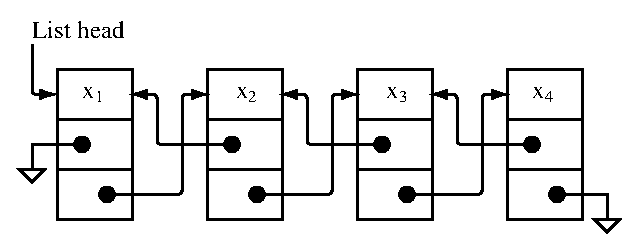
\includegraphics{dllist1}}
\caption{Doubly-linked list.}
\label{figure:dllist1}
\end{figure}

To implement the list, we'll split the operations into two parts: operations on list elements, and
operations on lists.  Given a list element, there are operations to get the next and previous
elements; and there are operations for inserting and removing elements from a list.

\begin{ocaml}
(* The type of elements in the list *)
type 'a elem

val nil_elem    : 'a elem
val create_elem : 'a -> 'a elem
val get         : 'a elem -> 'a
val prev_elem   : 'a elem -> 'a elem
val next_elem   : 'a elem -> 'a elem

(* The type of lists with elements of type 'a element *)
type 'a dllist

val create : unit -> 'a dllist
val insert : 'a dllist -> 'a elem -> unit
val remove : 'a dllist -> 'a elem -> unit
\end{ocaml}
%
The implementation starts with the list elements.  A link to an element can be null (at the end of
the list), or it can point to a real element.  Instead of having two kinds of links, we can fold the
two cases directly into the element type.  The list is designed to be modified in place, so the
links should be references to elements.

\begin{ocaml}
type 'a elem =
   Nil
 | Elem of 'a * 'a elem ref * 'a elem ref
\end{ocaml}
%
With this type definition in place, the implementation of elements is fairly straightforward.  A
fragment is shown below; the omitted functions are similar.

\begin{ocaml}
let nil_elem = Nil
let create_elem x = Elem (x, ref Nil, ref Nil)

let get = function
   Elem (x, _, _) -> x
 | Nil -> raise (Invalid_argument "get")

let prev_elem = function
   Elem (_, prev, _) -> !prev
 | Nil -> raise (Invalid_argument "prev_elem")
\end{ocaml}
%
Next, to implement the doubly-linked list, the list itself can be just be a reference to the first
element.  The function \hbox{\lstinline/create/} constructs an empty list, and \hbox{\lstinline/insert/} adds an
element at the head of the list.  The list operations are similar to what we would see on other
imperative languages; the links are modified in place as the list is changed.

\begin{ocaml}
type 'a dllist = 'a elem ref

let create () = ref Nil

let insert list elem =
   match elem, !list with
      Elem (_, prev, next), Nil ->
         prev := Nil;
         next := Nil;
         list := elem
    | Elem (_, prev1, next1), (Elem (_, prev2, _) as head) ->
         prev1 := Nil;
         next1 := head;
         prev2 := elem;
         list := elem
    | Nil, _ ->
         raise (Invalid_argument "insert")
\end{ocaml}
%
In the first case, the new element is added to an empty list; so both pointers are set
to \hbox{\lstinline/Nil/}.  In the second case, the list has a head element, which is modified so that its
previous link is now the new element.

Removing an element from the list is similar.  If the element to be removed is the head element,
then its previous link is \hbox{\lstinline/Nil/}, and the list must be updated to refer to the next
element.  Otherwise, the forward-link of the previous element must be adjusted.  Similarly, the
back-link of the next element must be adjusted.

\begin{ocaml}
let remove list elem =
   match elem with
      Elem (_, prev, next) ->
         (match !prev with
             Elem (_, _, prev_next) -> prev_next := !next
           | Nil -> list := !next);
         (match !next with
             Elem (_, next_prev, _) -> next_prev := !prev
           | Nil -> ())
    | Nil ->
         raise (Invalid_argument "remove")
\end{ocaml}

\labelsection{memoization}{Memoization}

\index{memoization}
Sometimes references and side-effects are used to improve performance without otherwise changing the
behavior of a program.  Memoization is an example of this, where a record is made of function
applications as a kind of run-time optimization.  If a function $f$ is pure, and $f(e)$ is computed
for some argument $e$, then any future computation $f(e)$ will return the same result.  When a
function $f$ is memoized, the results of function applications are stored in a table, and the
function is called at most once for any argument.

In OCaml, we can implement this in a generic way.  For immediate purposes, we'll represent the memo
(the table) as an association list.  The memoization itself can be implemented as a single higher-order function.

\begin{ocaml}
val memo : ('a -> 'b) -> ('a -> 'b)
\end{ocaml}
%
That is, the function \hbox{\lstinline/memo/} takes a function and returns a function with the same type.
The intent is that the result should be a function that is equivalent, but perhaps faster.  The memo
can be implemented as follows.

\begin{ocamlnum}
let memo f =
   let table = ref [] in
   let rec find_or_apply entries x =
      match entries with
         (x', y) :: _ when x' = x -> y
       | _ :: entries -> find_or_apply entries x
       | [] ->
          let y = f x in
          table := (x, y) :: !table;
          y
   in
   (fun x -> find_or_apply !table x)
\end{ocamlnum}
%
The memo table is defined as a mutable table on line 2; the table is filled in with argument/result
pairs as the function is called.  Given an argument \hbox{\lstinline/x/}, the
function \hbox{\lstinline/find_or_apply/} is called to search the table.  If a previous entry is found
(line 5), the previous value is returned.  Otherwise the function is called (line 8), the result is
saved in the table (line 9) by side-effect, and the value is returned.
Let's try it on a computation of Fibonacci numbers.

\begin{ocaml}
let rec fib = function
   0 | 1 as i -> i
 | i -> fib (i - 1) + fib (i - 2)
\end{ocaml}
%
To measure it, we can use the function \hbox{\lstinline/Sys.time/} to measure the CPU time taken by the process.

\begin{ocaml}
# let time f x =
   let start = Sys.time () in
   let y = f x in
   let finish = Sys.time () in
   Printf.printf "Elapsed time: %f seconds\n" (finish -. start);
   y
;;
@
\begin{topoutput}
val time : ('a -> 'b) -> 'a -> 'b = <fun>
\end{topoutput}
@
# let memo_fib = memo fib;;
@
\begin{topoutput}
val memo_fib : int -> int = <fun>
\end{topoutput}
@
# time memo_fib 40;;
@
\begin{topoutput}
Elapsed time: 14.581937 seconds
- : int = 102334155
\end{topoutput}
@
# time memo_fib 40;;
@
\begin{topoutput}
Elapsed time: 0.000009 seconds
- : int = 102334155
\end{topoutput}
@
\end{ocaml}
%
In the the first call, the computation of \hbox{\lstinline/fib 40/} took roughly 15 seconds, while the second
call was nearly instantaneous.

It should be noted that, although this kind of memoization does make use of side-effects, it has no
effect on results of the computation (as long as it is applied to pure functions).  In fact, if a
function $f$ is referentially transparent, so is \hbox{\lstinline/memo $f$/}---it behaves
as the original function, except that it trades space for time.

\labelsection{directed-graphs}{Graphs}

\index{graphs}
\index{minimum spanning tree}
\index{Kruskal's algorithm}
Let's finish this chapter with a classic algorithm from graph theory: Kruskal's algorithm for
minimum spanning trees.  Given a connected, undirected graph, a \emph{spanning tree} is a subset of
edges that forms a tree and includes every vertex.  If edges are assigned weights, the minimum
spanning tree is the spanning tree with the lowest weight.  The computation of minimum spanning
trees has many practical purposes.  One of the original uses was by Czech scientist Oscar
\misspelled{Bor\accent23{u}vka} in 1923 to minimize the cost of electrical coverage in Bohemia.

Kruskal's algorithm is specified as follows, for a weighted graph $(V, E)$ with vertices $V$ and
edges $E$.

\begin{enumerate}
\item Sort the edges $E$ by weight.
\item
For each edge in order of increasing weight, include the edge in the spanning tree if it would not form
a cycle with the edges already in the tree, otherwise discard it.
\end{enumerate}
%
The interesting part of the algorithm is step 2.  An example is shown in Figure~\ref{figure:kruskal}
for a small graph.  First, the two edges with weight 5 are added to the spanning tree.  Next, the
edges with weights 6 and 7 are added, but the edge with weight 8 is discarded because it would
produce a cycle.  Similarly, the edge with weight 9 is included, but the edge with weight 11 is
discarded, and the final edge 23 is discarded as well.

\begin{figure}
\centerline{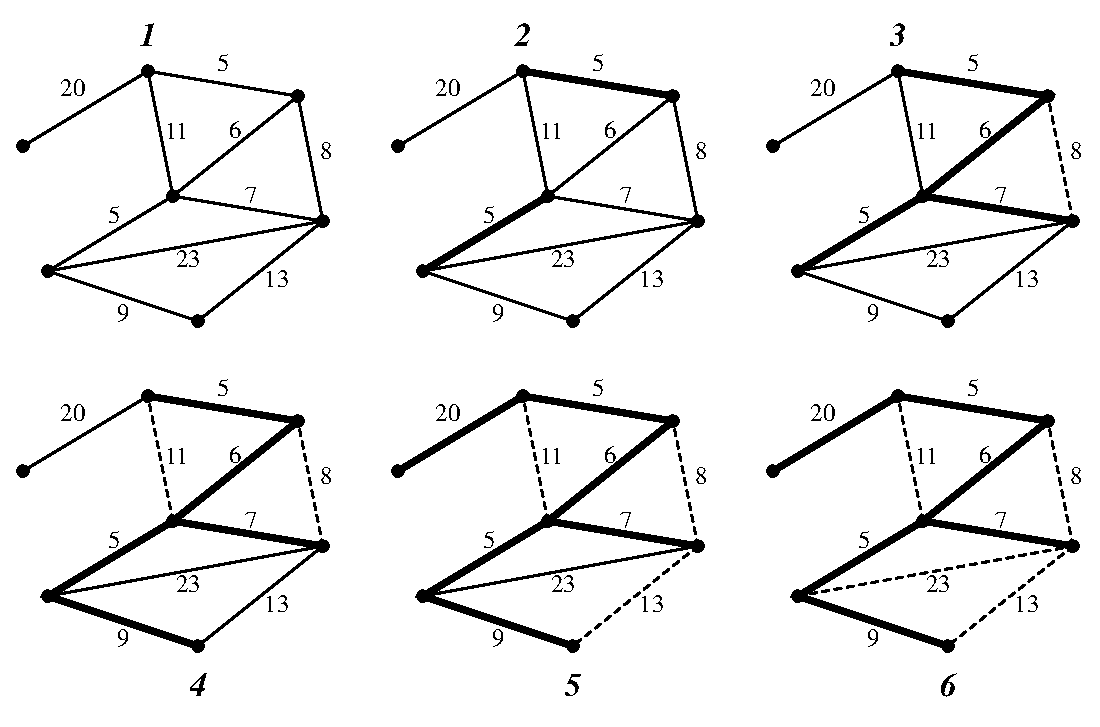
\includegraphics[scale=0.6]{kruskal}}
\caption{An example run of Kruskal's algorithm for computing the minimum spanning tree of a weighted undirected graph.}
\label{figure:kruskal}
\end{figure}

We can think of the algorithm as working over connected components of the graph.  When an edge
$(v_1, v_2)$ is included in the tree, the connected component containing $v_1$ is merged with the
component containing $v_2$.  In order to be included in the spanning tree, the vertices $v_1$ and
$v_2$ must belong to separate components---otherwise the edge would form a cycle.

We can implement this with a \emph{union-find} data structure, which supports two operations.

\begin{itemize}
\item
\lstinline/find : vertex -> vertex/,
where \hbox{\lstinline/find $v$/} returns a canonical vertex of the set (connected component) containing
$v$.  Two vertices $v_1$ and $v_2$ are in the same component if \hbox{\lstinline/find $v_1$ = find $v_2$/}.
\item
\lstinline/union : vertex -> vertex -> unit/,
where \hbox{\lstinline/union $u_1$ $u_2$/} takes the union of the sets containing canonical elements $u_1$ and $u_2$ (by side-effect).
\end{itemize}
%
Step 2 of Kruskal's algorithm can be written as follows, where the expression
%
\hbox{\lstinline/List.iter f edges/} calls the function \hbox{\lstinline/f/} for each edge in the list of edges.

\begin{ocaml}
(* An edge is a triple (weight, vertex1, vertex2) *)
type 'a edge = float * 'a vertex * 'a vertex

(* A list of edges, sorted by increasing weight *)
let kruskal edges =
   let spanning_tree = ref [] in
   List.iter (fun ((_, v1, v2) as edge) ->
      let u1 = find v1 in
      let u2 = find v2 in
      if u1 != u2 then begin
         (* v1 and v2 belong to different components *)
         spanning_tree := edge :: !spanning_tree;
         union u1 u2
      end) edges;
   !spanning_tree
\end{ocaml}
%
What remains is to specify the type for vertices, and to implement the functions \hbox{\lstinline/find/}
and \hbox{\lstinline/union/}.  One simple way to do so is to organize the vertices in each connected
component into a tree, where each vertex has a pointer to its parent.  The root of the tree is the
canonical element returned by the function \hbox{\lstinline/find/}.  Given roots \hbox{\lstinline/u1/}
and \hbox{\lstinline/u2/}, the union operation simply makes one a child of the other.
For efficiency, we use the following heuristics.

\begin{itemize}
\item When performing a \hbox{\lstinline/union/}, the smaller tree should become a child of the larger.
We'll save the size of the tree at the root.
\item
When performing a \hbox{\lstinline/find $v$/}, first find the root $u$, then traverse the path from $v$ to
$u$ a second time, updating all parent pointers to point to $u$.
\end{itemize}
%
Both heuristics will tend to make the tree fatter.  The second, called \emph{path compression},
decreases the cost of subsequent \hbox{\lstinline/find/} operations.

We'll represent a vertex as a pair \hbox{\lstinline/($\ms{label}$, $\ms{parent}$)/} where $\ms{label}$ is
the label of the vertex, and $\ms{parent}$ is the parent link: either \hbox{\lstinline/Root i/} for the
root vertex, or \hbox{\lstinline/Parent p/} if not.  The \hbox{\lstinline/union/} operation can be written as
follows.

\begin{ocaml}
type 'a parent =
   Root of int
 | Parent of 'a vertex

and 'a vertex = 'a * 'a parent ref

let union ((_, p1) as u1) ((_, p2) as u2) =
   match !p1, !p2 with
      Root size1, Root size2 when size1 > size2 ->
         p2 := Parent u1;
         p1 := Root (size1 + size2)
    | Root size1, Root size2 ->
         p1 := Parent u2;
         p2 := Root (size1 + size2)
    | _ ->
         raise (Invalid_argument "union: not roots")
\end{ocaml}
%
The \hbox{\lstinline/find/} operation is implemented in two parts: the actual find operation \hbox{\lstinline/simple_find/}, and the path compression \hbox{\lstinline/compress/}.

\begin{ocaml}
let rec compress root (_, p) =
   match !p with
      Root _ -> ()
    | Parent v -> p := Parent root; compress root v

let rec simple_find ((_, p) as v) =
   match !p with
      Root _ -> v
    | Parent v -> simple_find v

let find v =
   let root = simple_find v in
   compress root v;
   root
\end{ocaml}
%
It can be shown that with these heuristics, the complexity of step 2 of Kruskal's algorithm is $O((n
+ m) \alpha(n))$ where $n$ is the number of vertices $n = |V|$, $m$ is the number of edges $m =
|E|$, and $\alpha(n)$ is the inverse of Ackermann's function.  For any practical $n$, $\alpha(n)$ is
at most $4$, so Kruskal's algorithm effectively takes linear time.

The complexity argument is fairly long (see Kozen~\cite{Koz91} for a good explanation), but the key
benefit comes from path compression.  Suppose path compression were not used.  The first heuristic
would still ensure that path lengths are at most $\log n$ because the tree at least doubles in size
along each edge in the path from a vertex to the root of the tree, leading to a time complexity of
$O((n + m) \log n)$.  However, when path compression is used, the result of each \hbox{\lstinline/find/}
operation is effectively memoized, and the practical cost of the \hbox{\lstinline/find/} operation becomes
constant.

The principal motivation behind this example is to show that, in some cases, imperative programming
can be both simple and efficient.  While it is always possible to recode these algorithms in a pure
functional language, it is not always natural, and equivalent performance may not be achievable.

% -*-
% Local Variables:
% Mode: LaTeX
% fill-column: 100
% TeX-master: "paper"
% TeX-command-default: "LaTeX/dvips Interactive"
% End:
% -*-
% vim:tw=100:fo=tcq:
